\section{Introduction}

% 1.介绍 agent

% 1-1.引入 Agent 应用。
Large language models (LLMs) have evolved from chatbots to autonomous agents capable of exploring and solving complex tasks, such as programming~\citep{MBPP}, web search~\citep{WebGPT} and environment interaction~\citep{InterCode}.
% 1-2.介绍 Agent 请求的特点：多阶段，用户更注重完整的端到端时延，给现有的推理系统带来挑战。
Representative agent workflows, including ReAct~\citep{ReAct}, Plan-and-Solve~\citep{Plan-and-Solve}, Reflexion~\citep{Reflexion} and AgentFlow~\citep{AgentFlow}, typically execute an agentic request through multiple interdependent stages and LLM calls. 
As a result, users care about the end-to-end completion time of the entire workflow, which is often dominated by LLM generation, posing significant efficiency challenges for existing LLM inference systems.
% 1-3.我们的实验表明 Agent 应用的 LLM 请求在不同负载情况下瓶颈不同。
Our profiling reveals that the dominant latency bottleneck of agentic LLM requests varies with the concurrency. Under low concurrency, decode time dominates request latency, whereas queueing delay grows rapidly with increasing concurrency and eventually becomes the dominant latency component. 

% 2.介绍 SD

% 2-1.介绍 SD
Speculative decoding (SD) is a widely adopted technique to accelerate LLM decoding by generating candidate tokens with a lightweight drafting mechanism and verifying them in parallel with the target model~\citep{SD1,SD2,Eagle}. 
% 2-2.说明 Agent 场景下 SD 的机遇。
Agent workloads provide additional opportunities for speculative decoding due to their repetitive and structured generation patterns, such as recurring intermediate outputs, tool calls, and schema-constrained responses~\citep{SuffixDecoding,ToolSpec,AgentSpec}.
% 2-3.介绍 SD 的局限性。
However, the effectiveness of SD is highly sensitive to batch size. Previous studies have shown that SD speedup decreases as batch size increases and can eventually turn into performance degradation~\cite{SD-Speedup,SSSD,TurboSpec}. 
Our profiling of agent workloads reveals the same trend. In online agent serving, however, the running batch size varies substantially over time due to dynamic request arrivals and intermittent tool execution between LLM calls.

% 3.介绍现有的 Dynamic SD 
% 3-1.介绍 Dynamic SD 
Recent dynamic SD approaches adapt the draft length according to runtime signals such as batch size and token acceptance rate, and may reduce the draft length to zero when speculation is unfavorable~\cite{TurboSpec,SpecDec++,Nightjar}. 
% 3-2.说明 Dynamic SD 的局限性。
But these approaches perform adaptation internally within the speculative decoding framework rather than explicitly switching between native SD and non-SD execution paths. Our experiments show that such internal adaptation can still incur noticeable overhead compared with native non-SD execution.
Moreover, their systems typically rely on predefined switching policies, without exposing runtime control to external schedulers, which limits customized SD selection based on higher-level scheduling decisions.

% 4. 引入两个挑战
These observations raise two key challenges:
\begin{enumerate}
    % 如何更彻底地根据外部需求在 SD 和 NonSD 之间切换而不产生太多额外的开销
    \item \textbf{How to cleanly switch between SD and non-SD modes based on external decisions with less runtime overhead?}  
    % 在不同的并发度导致的瓶颈下如何降低 agent job 的端到端时延
    \item \textbf{How to reduce end-to-end latency under different concurrency with shifting latency bottlenecks?}
\end{enumerate}

% 系统架构图
\begin{figure}[t]
    \vspace{-30pt}
    \begin{center}
    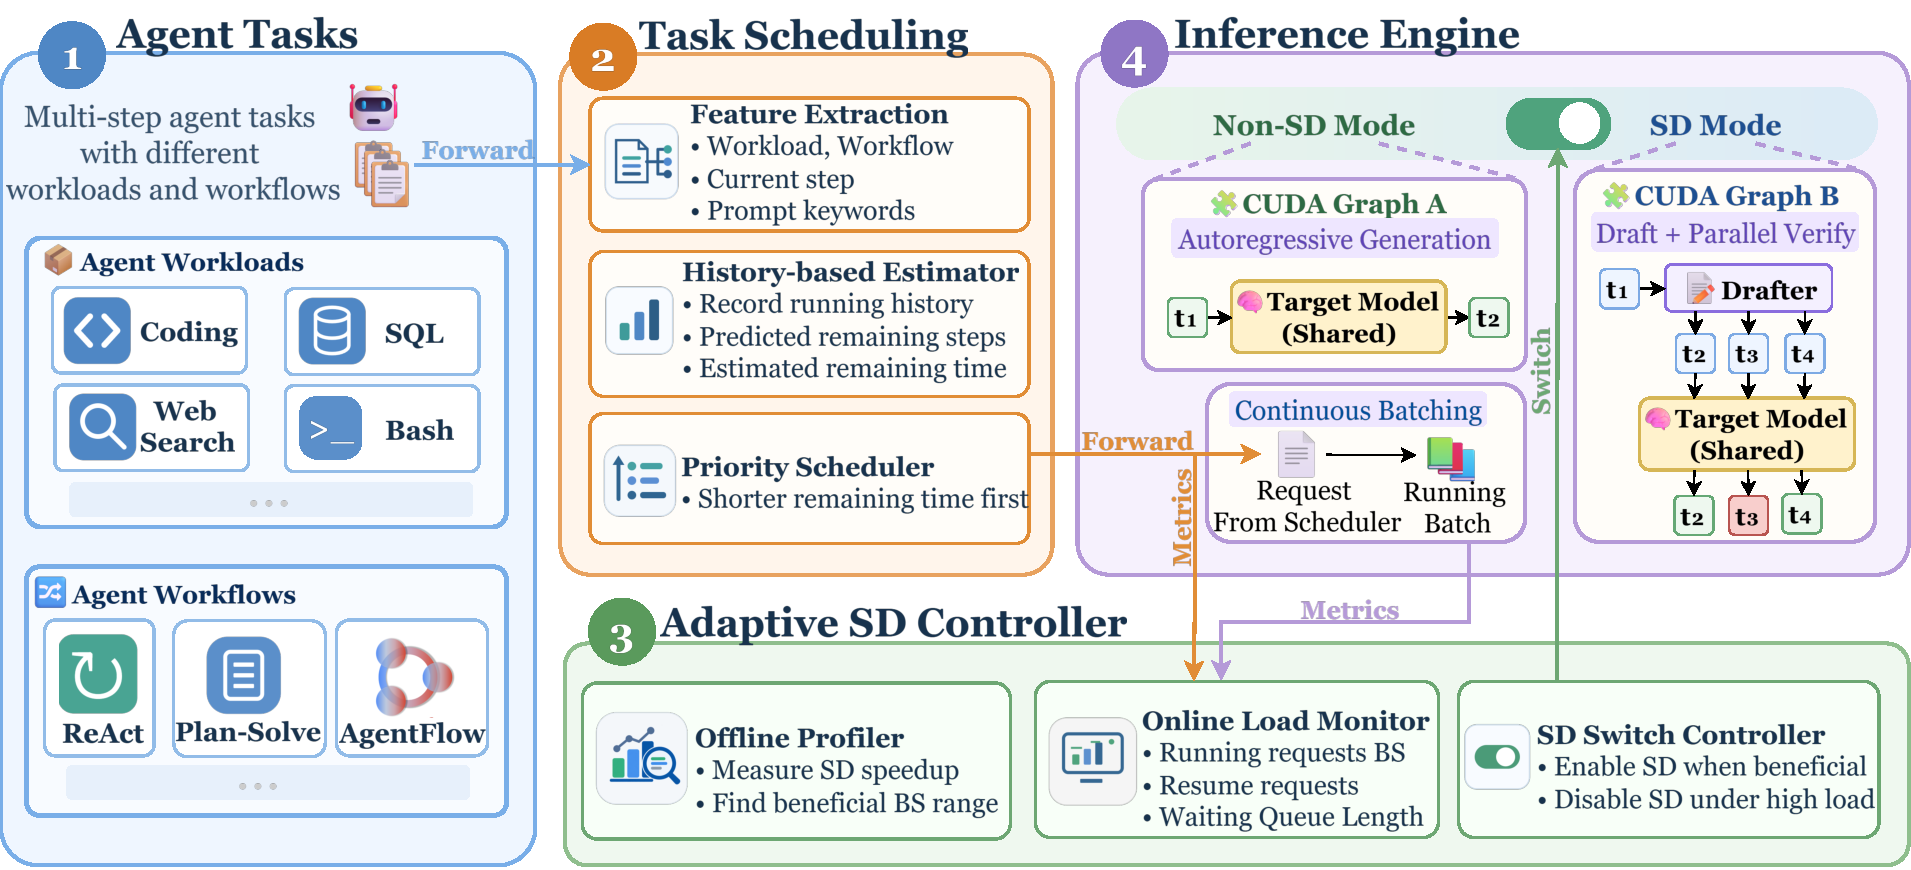
\includegraphics[width=0.9\linewidth]{figures/1-system overview.pdf}
    \end{center}
    \caption{Overview of SpecSys. SpecSys combines remaining-step-aware task scheduling with adaptive SD control. The scheduler estimates the remaining steps of agent jobs and prioritizes shorter jobs, while the SD controller selects between native SD and non-SD execution based on offline profiling and online serving load.}
    \label{fig:overview}
\end{figure}

% 5. 介绍我们的方法(SpecSys)
% 为了解决以上挑战，我们设计了 SpecSyS，引用系统架构图。
To address these challenges, we design SpecSys, an LLM inference system tailored for agent workloads, as shown in \autoref{fig:overview}. 
% SpecSys 在推理引擎的基础上开放了一个可供外部调用的切换开关，能够实现iteration级别的SD与NonSD的模式彻底切换。
Firstly, SpecSys extends the inference engine with an externally controllable switching interface, enabling complete iteration-level switching between native SD and non-SD execution modes.
% 为了降低 agent 任务的端到端时延，SpecSys 在不同的并发度根据不同的性能瓶颈设计了不同的策略。
To reduce the end-to-end latency of agent jobs, SpecSys employs different optimization strategies according to the dominant performance bottleneck under different concurrency.
% 在并发度较低时，SpecSys 会根据离线profile的数据评估 SD 加速比，选择性地调用上述接口启用或禁用 SD，以缓解Decode瓶颈。
Under low concurrency, SpecSys estimates the benefit of SD based on offline profiling results and selectively enables or disables SD through the aforementioned switching interface to alleviate the decoding bottleneck.
% 在并发度较高时，SpecSys 会根据 Agent 任务传入的workload，workflow，当前step，以及prompt中解析得到的关键词，使用历史记录分类查表的方式预测 Agent 任务的剩余 Step 数，然后贪心地选择哪些剩余 Step 数较低的任务，以缓解排队瓶颈。
Under high concurrency, SpecSys uses a lightweight history-based estimator to predict the remaining steps of each agent job based on its workload, workflow, current step, and prompt-derived keywords, and greedily prioritizes jobs with fewer predicted remaining steps to alleviate the queueing bottleneck.

Our contributions can be summarized as follows:
% 5-2. 列举 Contribution
\begin{itemize}
    % 彻底的可供外部调用的 SD-NonSD 切换接口。
    \item \textbf{Externally Controllable SD Switching.}
    We extend the inference engine with an externally controllable switching interface that enables complete iteration-level switching between native SD and non-SD execution modes, reducing runtime overhead by up to 71.3\%.
    % 轻量级的 Agent 任务剩余 Step 预测器。
    \item \textbf{Lightweight Agent Remaining-Step Prediction.}
    We design a lightweight history-based estimator that predicts the remaining steps of an agent job using its workload, workflow, current step, and prompt-derived keywords, achieving an average prediction accuracy of 84.1\% and recall of 82.2\%.
    % 基于并发度联合优化 Agent 任务调度和 SD 切换。
    \item \textbf{Load-Adaptive Agent Scheduling and SD Selection.}
    We selectively enable SD based on offline profiling under low concurrency, while disabling SD and prioritizing jobs with fewer predicted remaining steps under high concurrency.
\end{itemize}

% 6 概括实验
We conduct extensive evaluations of \textsc{SpecSys} across diverse online serving environments, three LLMs, four agent workloads, and three agent workflows. Compared with strong baselines, including ThunderAgent and vLLM with Dynamic SD, \textsc{SpecSys} reduces average job completion time (JCT), achieving from 1.18$\times$  to 2.10$\times$ speedup.